%% 
%% Copyright 2007-2020 Elsevier Ltd
%% 
%% This file is part of the 'Elsarticle Bundle'.
%% ---------------------------------------------
%% 
%% It may be distributed under the conditions of the LaTeX Project Public
%% License, either version 1.2 of this license or (at your option) any
%% later version.  The latest version of this license is in
%%    http://www.latex-project.org/lppl.txt
%% and version 1.2 or later is part of all distributions of LaTeX
%% version 1999/12/01 or later.
%% 
%% The list of all files belonging to the 'Elsarticle Bundle' is
%% given in the file `manifest.txt'.
%% 
%% Template article for Elsevier's document class `elsarticle'
%% with harvard style bibliographic references
\documentclass[12pt ,a4paper]{article}
%%%%%%%%%%%%%%%%%%%%%%%%%%%%%%%%%%%%%%%%%%%%%%%%%%%%%%%%%%%%%%%%%%%%%%%%%%%%%%%%%%%%%%%%%%%%%%%%%%%%%%%%%%%%%%%%%%%%%%%%%%%%

%% Use the option review to obtain double line spacing
%% \documentclass[authoryear,preprint,review,12pt]{elsarticle}

%% Use the options 1p,twocolumn; 3p; 3p,twocolumn; 5p; or 5p,twocolumn
%% for a journal layout:
%% \documentclass[final,1p,times,authoryear]{elsarticle}
% \documentclass[final,1p,times,twocolumn,authoryear]{elsarticle}
%% \documentclass[final,3p,times,authoryear]{elsarticle}
% \documentclass[final,3p,times,twocolumn,authoryear]{elsarticle}
%% \documentclass[final,5p,times,authoryear]{elsarticle}
%% \documentclass[final,5p,times,twocolumn,authoryear]{elsarticle}

\usepackage{amsmath}
\usepackage{amsfonts}
\usepackage{amssymb}
\usepackage[utf8]{inputenc}
\usepackage{url,hyperref,lineno,microtype,subcaption}
\usepackage{color,tensor,multirow,siunitx}
\usepackage[onehalfspacing]{setspace}
\usepackage{makecell}
\usepackage{graphicx}
\renewcommand{\cellalign}{cl}
% \usepackage{times}
\usepackage{caption}
\usepackage{lipsum}
\captionsetup[figure]{name=Fig., labelfont=bf}
\captionsetup[table]{name=Table, labelfont=bf}

\renewcommand{\cellalign}{cl}

\newcommand{\ds}{\displaystyle}
\newcommand{\nl}{\ \\ }
\newcommand{\ud}{\textrm{ d}}
\newcommand{\bs}{\bigskip}

\newcommand{\bu}{\mathbf{u}}
\newcommand{\bv}{\mathbf{v}}
\newcommand{\bx}{\mathbf{x}}
\newcommand{\be}{\mathbf{e}}
\newcommand{\bb}{\mathbf{b}}
\newcommand{\bk}{\mathbf{k}}
\newcommand{\bn}{\mathbf{n}}
\newcommand{\bR}{\mathbf{R}}

\definecolor{orange}{rgb}{1.0, 0.46, 0.09}
\definecolor{red}{rgb}{1,0,0}
\definecolor{blue}{rgb}{0,0,0.8}
\definecolor{green}{rgb}{0,0.5,0}
\newcommand{\emphc}[1]{\emph{\textcolor{red}{#1}}}
\newcommand{\hycom}{\textsc{hycom} }
\newcommand{\ie}{{\it i.e.}\ }
\newcommand{\eg}{{\it e.g.}\ }
\newcommand{\UV}{\mathbf{U}}
\newcommand{\todo}[1]{\textcolor{red}{TO DO: #1}}
\newcommand{\comment}[1]{\textcolor{orange}{#1}}
\usepackage[authoryear,round]{natbib}
\setlength{\bibsep}{0.0pt}
%\newcommand{\modif}[1]{\textcolor{blue}{#1}}
\renewcommand{\familydefault}{\sfdefault}
% \usepackage{times}

\begin{document}

\section{Coral reefs: a rich but threatened ecosystem}

Coral reefs are among the most productive and biologically diverse ecosystems on Earth \citep{connell1978diversity, moberg1999ecological} and supply food, income and coastal protection to vast numbers of people. Although they account for less than 0.5\% of the ocean floor \citep{spalding1997new}, almost a third of the known marine biodiversity is found on coral reefs \citep{moberg1999ecological}. Reef-related fisheries constitute around 10\% of the fish consumed by humans \citep{smith1978coral} and hundreds of millions of people depend on coral reefs for their livelihood or part of their protein intake \citep{salvat1992coral,hoegh2019people}. Through calcification, corals create the structure of a complex three-dimensional habitat that serves as spawning, breeding and feeding area for many species \citep{moberg1999ecological}. This complex reef framework  dissipates waves, protecting shorelines from currents and storms and preventing land loss due to erosion \citep{ferrario2014effectiveness,elliff2017coral}. Additionally, wave dissipation creates lagoon and sedimentary environment, providing favorable conditions for the growth of seagrass and mangrove ecosystems \citep{moberg1999ecological}.

The calcifying process of reef building corals heavily depends on their symbiosis with the microalgae zooxanthellae. These unicellular symbionts convert sunlight and carbon dioxide into organic carbon and oxygen, providing the coral host with most of the energy needed to meet its metabolic demands \citep{muscatine1977reef}. However, adverse environmental conditions such as elevated sea surface temperature can cause damage to the mechanisms maintaining this association, resulting in the expulsion of the endosymbionts \citep{hoegh2007coral}. This process, called bleaching, causes the coral to loose their pigmentation and reveals their underlying white skeleton \citep{baker2008climate}. Bleached corals are physiologically and nutritionally compromised, and prolonged bleaching over several months leads to high coral mortality \citep{hughes2018spatial}. Decline in coral health and cover pushes the reef ecosystem to a macroalgal-dominated state \citep{hughes2003climate,mumby2007thresholds}. Once a "tipping point" is exceeded, returning to a coral-dominated state becomes difficult \citep{mumby2007thresholds,graham2015predicting}.

Despite their importance, coral reefs have experienced a massive system-wide decline \citep{hoegh2017coral}: it is estimated  that 30\% have already been severely damaged, and close to 60\% may be lost by 2030 \citep{hughes2003climate}. This global decline in live coral cover \citep{gardner2003long,pandolfi2003global,bruno2007regional} is caused by both global and local anthropogenic stressors. The main global stressor is climate change induced ocean warming, that cause recurrent mass bleaching events at an increasing frequency \citep{connell199730, hughes2018spatial}. Furthermore, thermal stress can increase the susceptibility of corals to disease, leading to an increase in the incidence of coral outbreaks \citep{harvell2002climate,bruno2007thermal,muller2012caribbean}. Local stressors are numerous and include pollution \citep{loya1980effects}, coastal development \citep{erftemeijer2012environmental, cunning2019extensive}, nutrient run-off \citep{hughes2003climate,sheppard2017biology}, and overfishing of herbivorous species controlling algae growth \citep{jackson2001historical}.

Due to the combined damages from of all these stressors, it is now impossible to return reefs to their past configurations \citep{hughes2017coral}. Instead, the challenge is now to maintain the biological functions of coral reefs through quickly changing environmental conditions. This will require to rapidly address greenhouse gas emissions, as well as local actions to boost the capacity of coral reef ecosystems to survive climate change \citep{hughes2003climate,knowlton2008shifting,graham2015predicting}. The aim of the present dissertation was therefore to use modeling tools to better understand the drivers of coral demise and hence inform such local actions to support ecosystem management in Florida, the third largest barrier reef of the world.

\section{Identifying the threats to coral survival in \\Florida}

The Florida Reef Tract (FRT) spans over approximately 577 km from the Dry Tortugas (DRTO) west of the Florida Keys to the St. Lucie Inlet in Martin County, constituting the third largest barrier reef in the world \citep{finkl2008shelf}. These reefs have a fauna and species richness typical of Caribbean reefs, including more than 40 species of stony corals \citep{banks2008reef,jackson2014status}. The northern half-section of the FRT consists of relic, Holocene framework reefs and indurated sand ridges harboring a rich but non-framebuilding fauna. Reefs in this area are separated into three shore-parallel reefs (inner, middle, outer) separated by sandy plains. Benthic cover is generally denser on the middle and outer reefs while the inner reef harbors some large patches of dense \textit{Acropora cervicornis}. The dominant reef builder is the bouldering \textit{Montastraea cavernosa} but living hard coral cover is pretty low (below 6\%) \citep{banks2008reef}. The southern half-section isa chain of limestone islands (the Keys) that extend from the southern tip of the Florida mainland southwest to the DRTO. The Upper Keys are remnants of ancient coral reefs and the Lower Keys are sand bars \citep{hoffmeister1968geology}. The DRTO are made of small circular reef banks whose coral populations are among the most preserved of the continental United States \citep{hine2008coral, kourafalou2018physical}. Moreover, they are believed to be important sources of recruitment for coral-reef fishes in the Florida Keys \citep{domeier2004potential}. 

\todo{Add figure with map of the FRT}

Florida's Coral Reef (FCR) is of considerable importance to the economy of the state. \cite{johns2003socio} estimated the contribution of recreational users of natural and artificial reefs over the period June 2000 to May 2001 to have been US\$2.3 billions in sales and US\$1.1 billion in income. Moreover, recreational use of the reefs was evaluated to bring 36,500 full and part-time jobs. Focusing on natural reefs only, \cite{brander2013total} estimated the total coral reef values Florida to be US\$174 millions. However, this value might be underestimated as non-use value and indirect use values, such as support for coastal fisheries \citep{ault2006building} and coastal protection \citep{ferrario2014effectiveness} were not taken into account.

Nevertheless, FCR has been heavily impacted by the human activities of the major metropolitan area of greater Miami. These impacts include densely populated coastlines, high visitor numbers, polluted terrestrial run-off and overfishing \citep{jackson2014status}. For example, dredging operations during the PortMiami Deep Dredge Project (PMDDP) was reported to cause the death of $>$560,000 corals \citep{cunning2019extensive}. Florida's coral reefs have therefore declined significantly over the past decades due to anthropogenic stressors and numerous disease outbreaks \citep{gardner2003long, jackson2014status}. Populations of previously dominant reef-building acroporids almost totally disappeared throughout the Caribbean and Florida \citep{aronson2001white}, and coral cover dropped from 40 to 60\% in 1975 to $<$7\% in the Florida Keys \citep{jackson2014status} and $<$3\% in the northern section of the FRT \citep{walton2018impacts}. Furthermore, since 2014, many coral species have experienced widespread and severe decline caused by the ongoing outbreak of stony coral tissue loss disease (SCTLD). For instance, the abundance \textit{M. cavernosa}, once one of the most abundant species of the FRT, decreased by 45\% between 2015 and 2016 \citep{walton2018impacts}.

Coral disease outbreaks are frequent in the Caribbean, which is considered a disease "hot spot" because of the fast emergence, high prevalence, wide geographic distribution, and virulence of coral diseases in the area \citep{green2000significance, harvell2007coral}. For instance, populations of  \textit{Acropora} spp. decreased by $>$95\% throughout the Caribbean during numerous outbreaks of white-band disease in the 1970-1990s \citep{aronson2001white}. Other ajor outbreaks include the white plague and black band diseases, that respectively affect 22 and 42 corals species and caused significant declines in reef-building coral populations in the Caribbean \citep{bruckner2003field,miller2009coral, muller2011black}. 

The latest major outbreak affecting coral reefs of the Caribbean is the SCTLD \citep{noaa2018}. First observed off the coasts of Miami in 2014 during the PMDDP \citep{precht2016unprecedented}, the disease has since spread throughout the entire Florida Reef Tract and numerous territories of the Caribbean \citep{alvarez2019rapid, kramer2019map, estrada2021effects}. The outbreak affects at least 24 species of scleractinian coral and often results in whole colony mortality \citep{precht2016unprecedented, walton2018impacts}. Briefly, the gross morphology of SCTLD can be focal or multifocal, with locally extensive to diffuse areas of acute to subacute tissue loss distributed basally, peripherally, or both. In some cases, tissues bordering areas of chronic tissue loss show indistinct bands (1–5 cm) of pallor, progressing to normal pigmentation away from the denuded skeleton. The continued persistence of the outbreak, the high number of species affected, and its large geographical distribution of reports consistent with the case definition suggests that SCTLD is the largest coral disease outbreak on record in Florida. Although the causative agent of the disease remains unknown, hydrodynamics are likely to play an important role in its propagation as both modeling studies and ex situ experiments show evidence of waterborne disease transmission \citep{aeby2019pathogenesis,dobbelaere2020coupled,eaton2021measuring,meiling2021variable}. Furthermore, recent studies showed evidence that sediments can act as a vector for the SCTLD \citep{rosales2020rhodobacterales, studivan2022reef}. 

\todo{Add figure with pictures of SCTLD.}

Additionally, Florida is a prime landfall target for tropical cyclones from June through November (Fig. \ref{inro:landfall}). Hurricanes that forms in June and July are usually weak while hurricanes occurring in August and September tend to become severe storms \citep{banks2008reef}. This is illustrated by Hurricane Irma, one of the strongest and costliest hurricanes on record in the Atlantic, that made landfall in Florida in September 2017 as a category 4 hurricane \citep{irmaNOAA, xian2018brief}. Hurricanes are a major agent of coral mortality in the Caribbean that contributed to teh decline of acroporids \citep{gardner2003long,aronson2001white}. They cause a wholesale destruction of the reef biota on their passage and can induced coral burial through sediment resuspension \citep{banks2008reef, miller2008effects}. Furthermore, they significantly impact the content of surface waters through upwelling and mixing, which can disturb the benthic communities \citep{wachnicka2019hurricane,varlas2020investigating}. Furthermore, these 

\begin{figure}
    \centering
    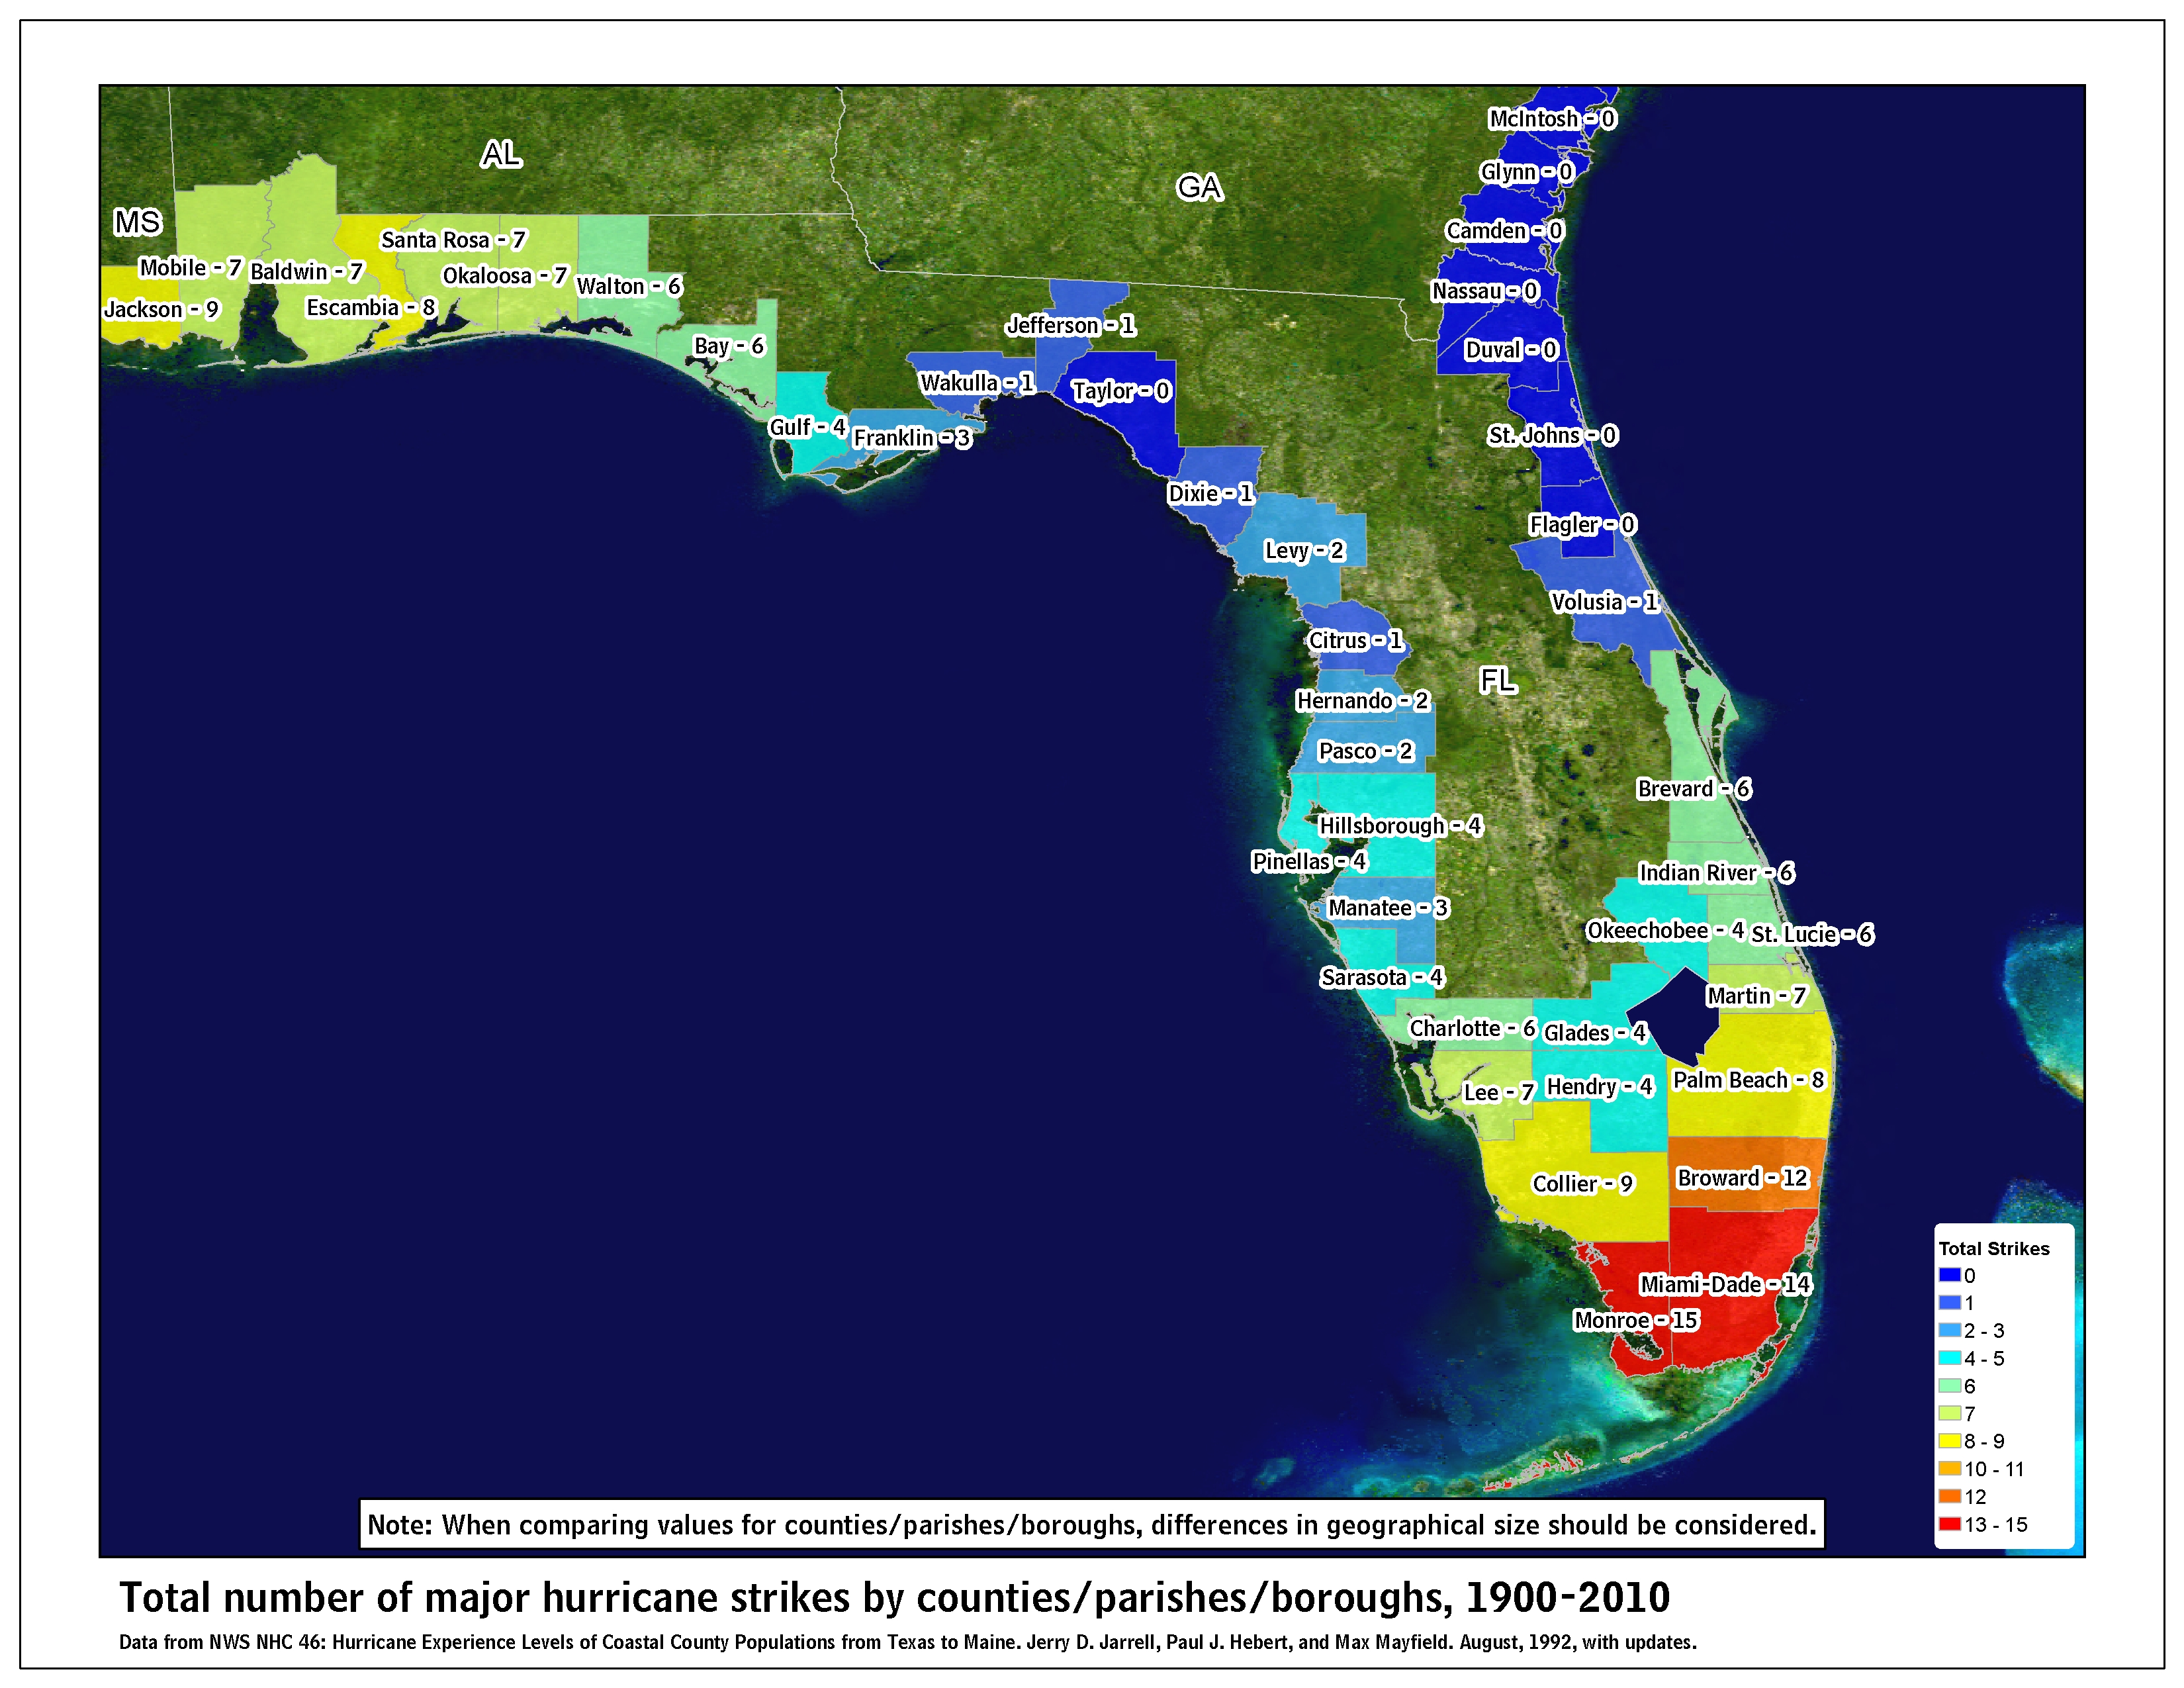
\includegraphics[width=\textwidth]{figures/hurricane_strikes.jpg}
    \caption{}
    \label{inro:landfall}
\end{figure}

\section{Thesis objectives}

\section{Modeling the hydrodynamics of the FRT}



\bibliographystyle{apalike} 
\bibliography{./biblio.bib}

\end{document}